\section{Energetic particles in the heliosphere}
\label{sec:particles_heliosphere}

\begin{figure}
	\centering
	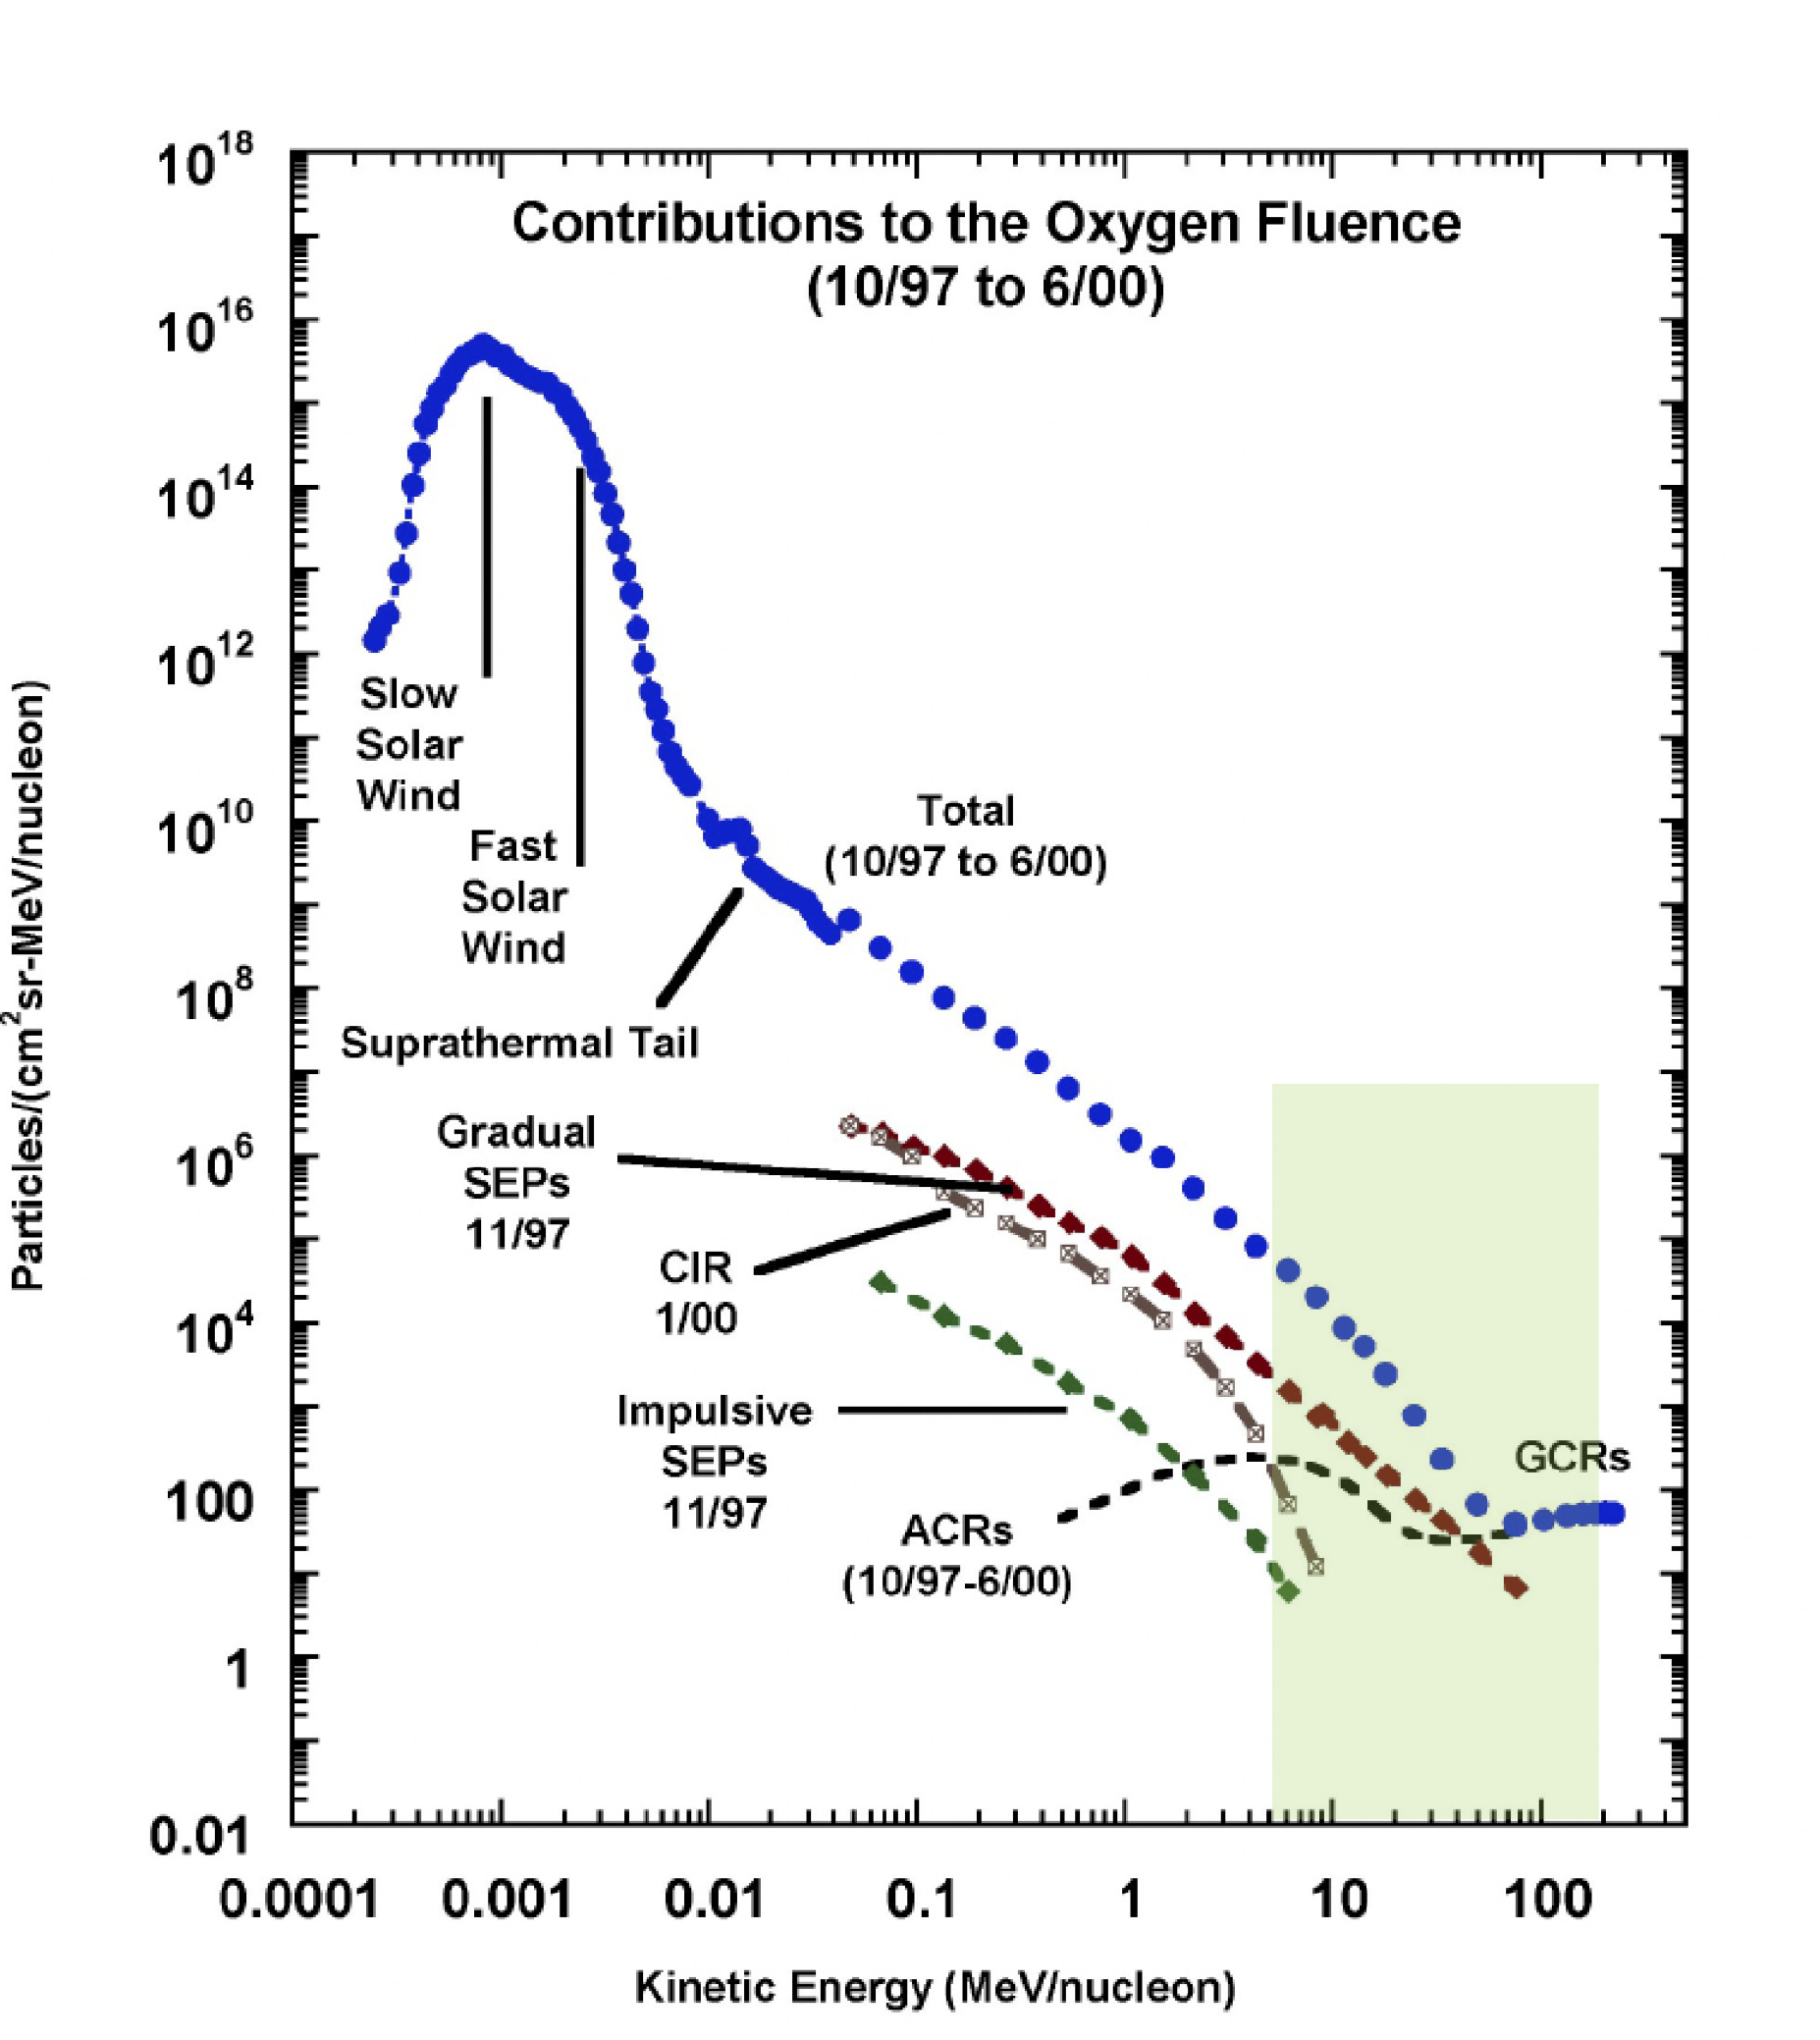
\includegraphics[width = 0.8\textwidth]{images/heliospheric_particle_spectra_color.png}
	\caption[Energy spectra of oxygen ions in near-Earth space]{The typical oxygen spectra in the interplanetary space near Earth, indicating the contributions of different particle populations, particularly in the energy range between few MeV/nuc and few hundreds MeV/nuc (shadow region), where \acs{SEP}, \acs{ACR} and \acs{GCR} coexist. The spectra of other particles species such as, helium and proton have the similar shape but a different flux level in corresponding energy region. The figure is adapted from \citep{Mewaldt-2001}}
	\label{Fig:Oxygen_spectra_heliosphere}
\end{figure}

Heliosphere is a vast, bubble-like region in the space that envelops the Sun. This region is moving in the \ac{ISM} with a speed of about 25 km/s \citep{McComas2015ApJS}. Such a cavity is created by the sun and governd by its magnetic field and solar wind; a substantial amount of plasmas of various particle populations fill this space. The particle populations could be identified from Fig.\ref{Fig:Oxygen_spectra_heliosphere} which is adapted from \citet{Mewaldt-2001}. Based on the accumulated measurement of oxygen by \ac{ACE} between 1997 and 2000, the fluence oxygen spectrum which spans over more than 7 orders of magnitude from keV/nuc to GeV/nuc provides clear insight into the lower energy particles including slow solar wind, fast solar wind, suprathermal tail, and high energy particles composed of \ac{SEP}, \ac{ACR}, and the extremely high energy \ac{GCR}. 
Among them \acs{GCR} originate from distant sources outside the solar system, while \acs{ACR} sources located near the boundary of heliosphere. The remaining energetic particles are the parrticle accelerated and generated inside of the heliosphere at the multiple locations, including solar surface, interplanetary space and even the planet for instance Jupiter.

Solar wind is a stream of charged particles released from the solar corona, the upper atmosphere of the Sun. Such a group of plasam consists of mainly protons and electrons that continously flow outward and expend to about $\sim$ 100 au (differ in directions). The typical energy range of the solar wind is between 0.5 keV and 10 keV. Depending on the locations on the sun that produces the solar wind, the speed and density of solar wind might be different. For instance the fast solar wind with a typical speed between 500 and 800 kilemeters per second emits from the coronal holes which are funnel-like regions of open field lines in the magnetic field and usually appear in the north and south pole of sun. Therefore, the fast solar dominate the high latitude regions. While the slow solar wind is observed to have a velocity of about 300 - 500 kilometers per second and is believed to originate from the streamer belt along the equatorial belt. The slow solar wind is more likely to be observed in the low latitude regions.

%plasma embedding with magnetic field

Suprathermal particles are charged ions and electrons that move about two to hundreds times faster than the solar wind particles. In the spectrum shown in Fig.\ref{Fig:Oxygen_spectra_heliosphere}, the suprathermal particles are beyond the tails of the fast solar wind and are the dominate particles between few keV to hundreds of keV. The source of suprathermal particle might be the accelerated solar wind and the remanent of the previous solar eruptions and \ac{SEP} events. Those particles play am important role in contributing seed particles for the \ac{SEP} events.

Above the energy of suprathermal particle are the energy range that we are interested in this thesis, especially the energy range between 10 MeV/nuc and few hundred MeV/nuc where the dominated particles are \ac{SEP} (not limited to this energy range),\ac{ACR} (up to $\sim$ 100 MeV/nuc) and lower energy \ac{GCR}. The measurements we used in this study are from this energy range.

The \ac{SEP} are the high energetic particles with energy of few keV up to $\sim$ GeV oriented from the sun and accelerated during the solar activities like solar flare and \ac{CME} driven shocks. \acs{SEP} events are recurring, short term, and intensive. Different type of \acs{SEP} events persist for different time scales from few hours to few days. Such high energy particles are one of the major threats in the space.
%also particle from solar, accelerated by different mechanism. The enery range of \ac{SEP} are quite broad, especially depending the on where the measurement carried on. Recently \ac{SOLO} and \ac{PSP} frequently measure the hundreds keV \ac{SEP}.

\acs{ACR} are the high energy interstellar pick-up ions \citep{Giacalone2022SSRv} which are ionized neutral interstellar atoms generated by solar UV radiation after they move cross the boundary and enter the heliosphere. Those ionizing particle are then carried by the expanding solar wind to the outer boundary of helioesphere, where they are accelerated by the termination shock and then propagate inwards. The typcial \ac{ACR} species that have been observed are proton, helium, oxygen, nitrogen, iron, neon. 

\ac{GCR} are the fully ionized particles that is accelerated at the so-called supernova remnants \citep{Blasi2013AARv2013} which are outside of the solar system. Those high energy particles bombard Earth in a constant and slowly varying way. The complete GCR spectrum cover the energy from typical 1MeV \citep{Potgieter2013LRSP} to ZeV which is larger than the energy range in Fig.~\ref{Fig:Oxygen_spectra_heliosphere}. The \acs{GCR} is comprised of about 89\% of hydrogen, 10\% of helium, 1\% of heavier ions as well as electron, positron and antiprotons. 

After entering the heliosphere, the transport of both cosmic rays are controled by the \ac{HMF}, hence \ac{ACR} and \ac{GCR}'s temporal variaton is highly related with the solar activities and the so-called solar modulation, which periodcally changes in 11 and 22 year periods. 


\section{Solar energetic particles}

\subsection{Two types of SEPs}

\begin{figure}[!htb]
	\centering
	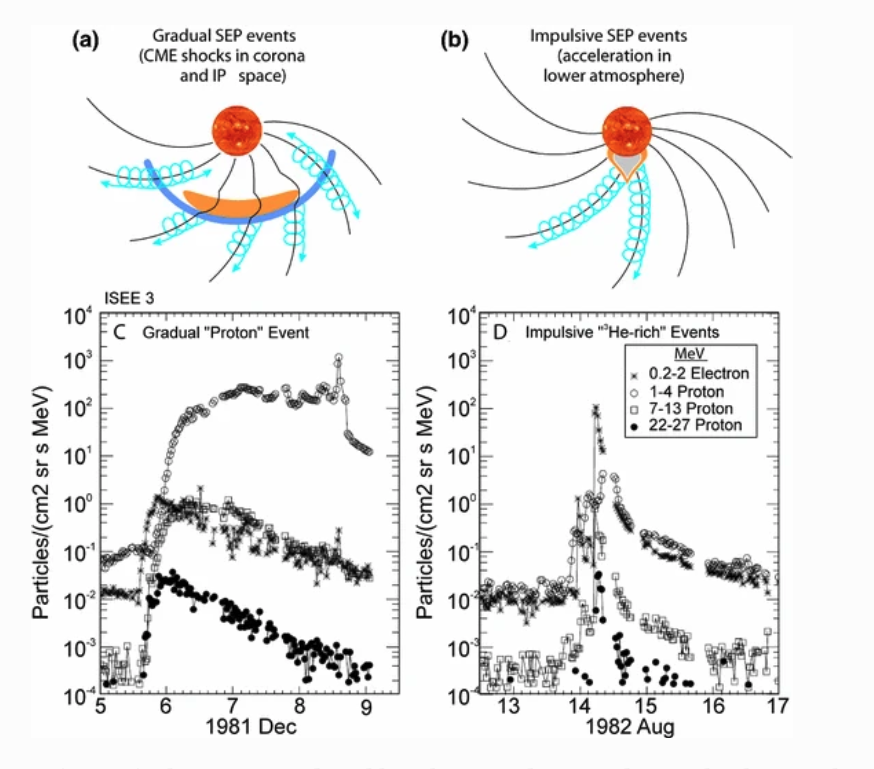
\includegraphics[width = 0.75\textwidth]{images/SEP_two_type.png}
	\caption[Two types of Solar energetic particle (SEP) event]{Two classes of \ac{SEP} events. (a) The gradual \ac{SEP} events that are associated with the CME drivens shocks in the coronal or in the interplanetary space and the particles populate the \ac{IMF} lines over a wide range of longitudes. (b) The impulsive SEP event that is associated with the solar flares and the particles only populate a limited range of the open \ac{IMF} lines that are well-connected to the flare site. Plots (c) and (d) are the corresonpding typical proton and electron time profile of the large gradual and small impulsive SEP events. The figure is reproduced from \citet{Desai_Diacalone2016LRSP}.}
	\label{Fig:two_type_SEP}
\end{figure}
The first observation of \ac{SEP} events was made back to a magnetic storm on March 1, 1942 \citep{lange1942note,forbush1942further}, during which three unusual increase in the cosmic-ray intensity was observed on ground-based ionization chambers and the neutron monitors and appeared simultanously with the solar flare eruption. Later, \citet{Forbush1946} attributed such increases to the charged particles oriented from the sun with sufficient energy to penetrate the Earth's atmosphere. Now we have known that this is the so-called \ac{GLE}, one type of the most hazard energetic particles in the space of more than 433 MeV/nuc energy, typical more than GeV. \citep{meyer1956solar,Shea2012SSRv,gopalswamy2013first,thakur2014ground, Reames2013, Mironshnichenko2013Ge}.

It is commonly believed that the generation of \acp{SEP} are highly related to the solar flare during first few decades after the discovery of \ac{SEP} because they appeared simultanously. This is the so-called "solar flare myth" as discussed in \citep{gosling1993the}.  The important role of \ac{CME} and its driven shocks in the generation of \ac{SEP} was largely underestimated, though a quite lot researches on the characters of such \acp{SEP} like the duration, longitudinal distribution, the abundance of the typical elements and their association with radio burst had already indicated the existence of two types of distinct events - impulsive and gradual \ac{SEP} events \citep{kahler1978prompt,kahler1984associations,cliver1982injection,cane1986two, reames1988ApJ}.
Currently, the scientists have generated such a classic two-class paradigm (See,Fig.~\ref{Fig:two_type_SEP} and Tab.~\ref{Tab:Two_type_SEP}) which has been widely accepted by the science community \citep{kallenrode2003current, reames2013two,Desai_Diacalone2016LRSP, Reames2021LNP}. Both acceleration mechanisam and the source locations are different for two type of \acp{SEP}.


Fig.~\ref{Fig:two_type_SEP} illustrates the current scenario of gradual (left) and impulsive (right) \acp{SEP}.
The gradual events are diffusively accelerated by the CME-driven coronal and interplanetary (IP) shocks. Generally, a complete gradual \ac{SEP} event usually consists of an sharp increase phase as the start, a long lasting plateau and a flux peak at lower energy which indicates the arrival of \ac{CME} at the detector. The event finishs with a decay phase and flux return to the quite level. The whole process might persist from one day to several days. Gradual \ac{SEP} is always accompanied by the type II radio burst, which is a broad and slow shift struture in the radio dynamic spectrum and is considered as a signature of \acp{CME} and the propagtion track of \ac{CME} from the sun to 1 au. Shocks mainly accelerate protons and heavy ions, but not electrons with the same efficiency, causing the smaller electron to proton ratio compared with impulsive \ac{SEP}. Besides, the gradual \ac{SEP} spread widely in the IP since \ac{CME} has broader longitude extent and can be measured by multiple detectors even if they are far away from each other. In the next section, we will discuss more about the widespread event. The appearance frequency of gradual \ac{SEP} during the solar maximum is about $\sim 100$ per year.

While the solar flare which erupts from the solar active region is considered as the souce of the impulsive \ac{SEP} event. The fierce magnetic reconnections happened during the flare eruption can accelerate particles, especially electons, up to hundred MeV. Therefore, the electrons are the dominant particles in such event. Besides, in this senario, the particles escape from the open magnetic field and arrive at the Earth along the spiral magnetic field. i.e. Parker spiral, \citep{Parker-1958} that is shaped by the expanding solar wind. From the Earth's point of view, the impulsive \acp{SEP} are typically located in a narrow region in the west hemisphere of sun. Type III radio burst usually appears with impulsive event, rather than \ac{CME}.
The appearance frequency of impulsive \ac{SEP} during the solar maximum is about $\sim 10^3$ per year. The typical duration of impulsive \ac{SEP} is less than days.

It is worth noting that, \citep{cane2003two} proposed a type of mixed event that have flare particles as seed population and later those particles are reaccelerated by the shocks. Such intensive \acp{SEP} have two components related both flare and shocks.  %[Might find a paper and confirm the statements] 
In Tab.~\ref{Tab:Two_type_SEP}, we summarized the general properties of the two types of \ac{SEP} events.

\begin{table}{!h}
	\centering
	\caption[Two classes of SEP events]{Two-class paradigm of \ac{SEP} event, adapted from \citet{kallenrode2003current,	Desai_Diacalone2016LRSP, Wang2009}.}
	\begin{tabular}{c|c|c}
		\hline
		\hline
		Property 	& Gradual \ac{SEP} 	& Impulsive \ac{SEP} \\
					& (Large \ac{SEP})	& (Electron/$^3$He-rich \ac{SEP}) \\
		\hline
		Dominant particle	& proton	& electrons \\
		Electron/proton ration &  50 - 100 &  $10^2 - 10^4$  \\
		$^3$He/$^4$He ratio	& 4$\times$ 10$^-4$ & 1 \\
		Fe/O			& $\sim$ 0.1			& $\sim$ 1	 \\
		H/He		 	& $\sim$ 100			& $\sim$ 10 \\
		Q$_{Fe}$		& $\sim$ 14 			& $\sim$ 20 \\
		Duration		& $\sim$ Days			& $\sim$ hours \\
		Longitude cone	& $>$ 100 $^\circ$		& $<$ 30$^\circ$ \\
		Seed particles	& Ambient Corona or Solar wind & Heated corona \\
		Radio type		& Type II/IV	& Type III \\
		X-ray duration	& $\sim$ hours	& $\sim$ minutes - 1h \\
		CME association	& Fast/halo CME	& No	\\
		Frequency(at 	& $\sim$ 10	& $\sim$ 1000 \\
		solar maximum)	& 	& 	\\
		\hline
	\end{tabular}
	\label{Tab:Two_type_SEP}
\end{table}


\subsection{Wide-spread SEP and multi-instruments observation}


\begin{figure}[!htbp]
	\centering
	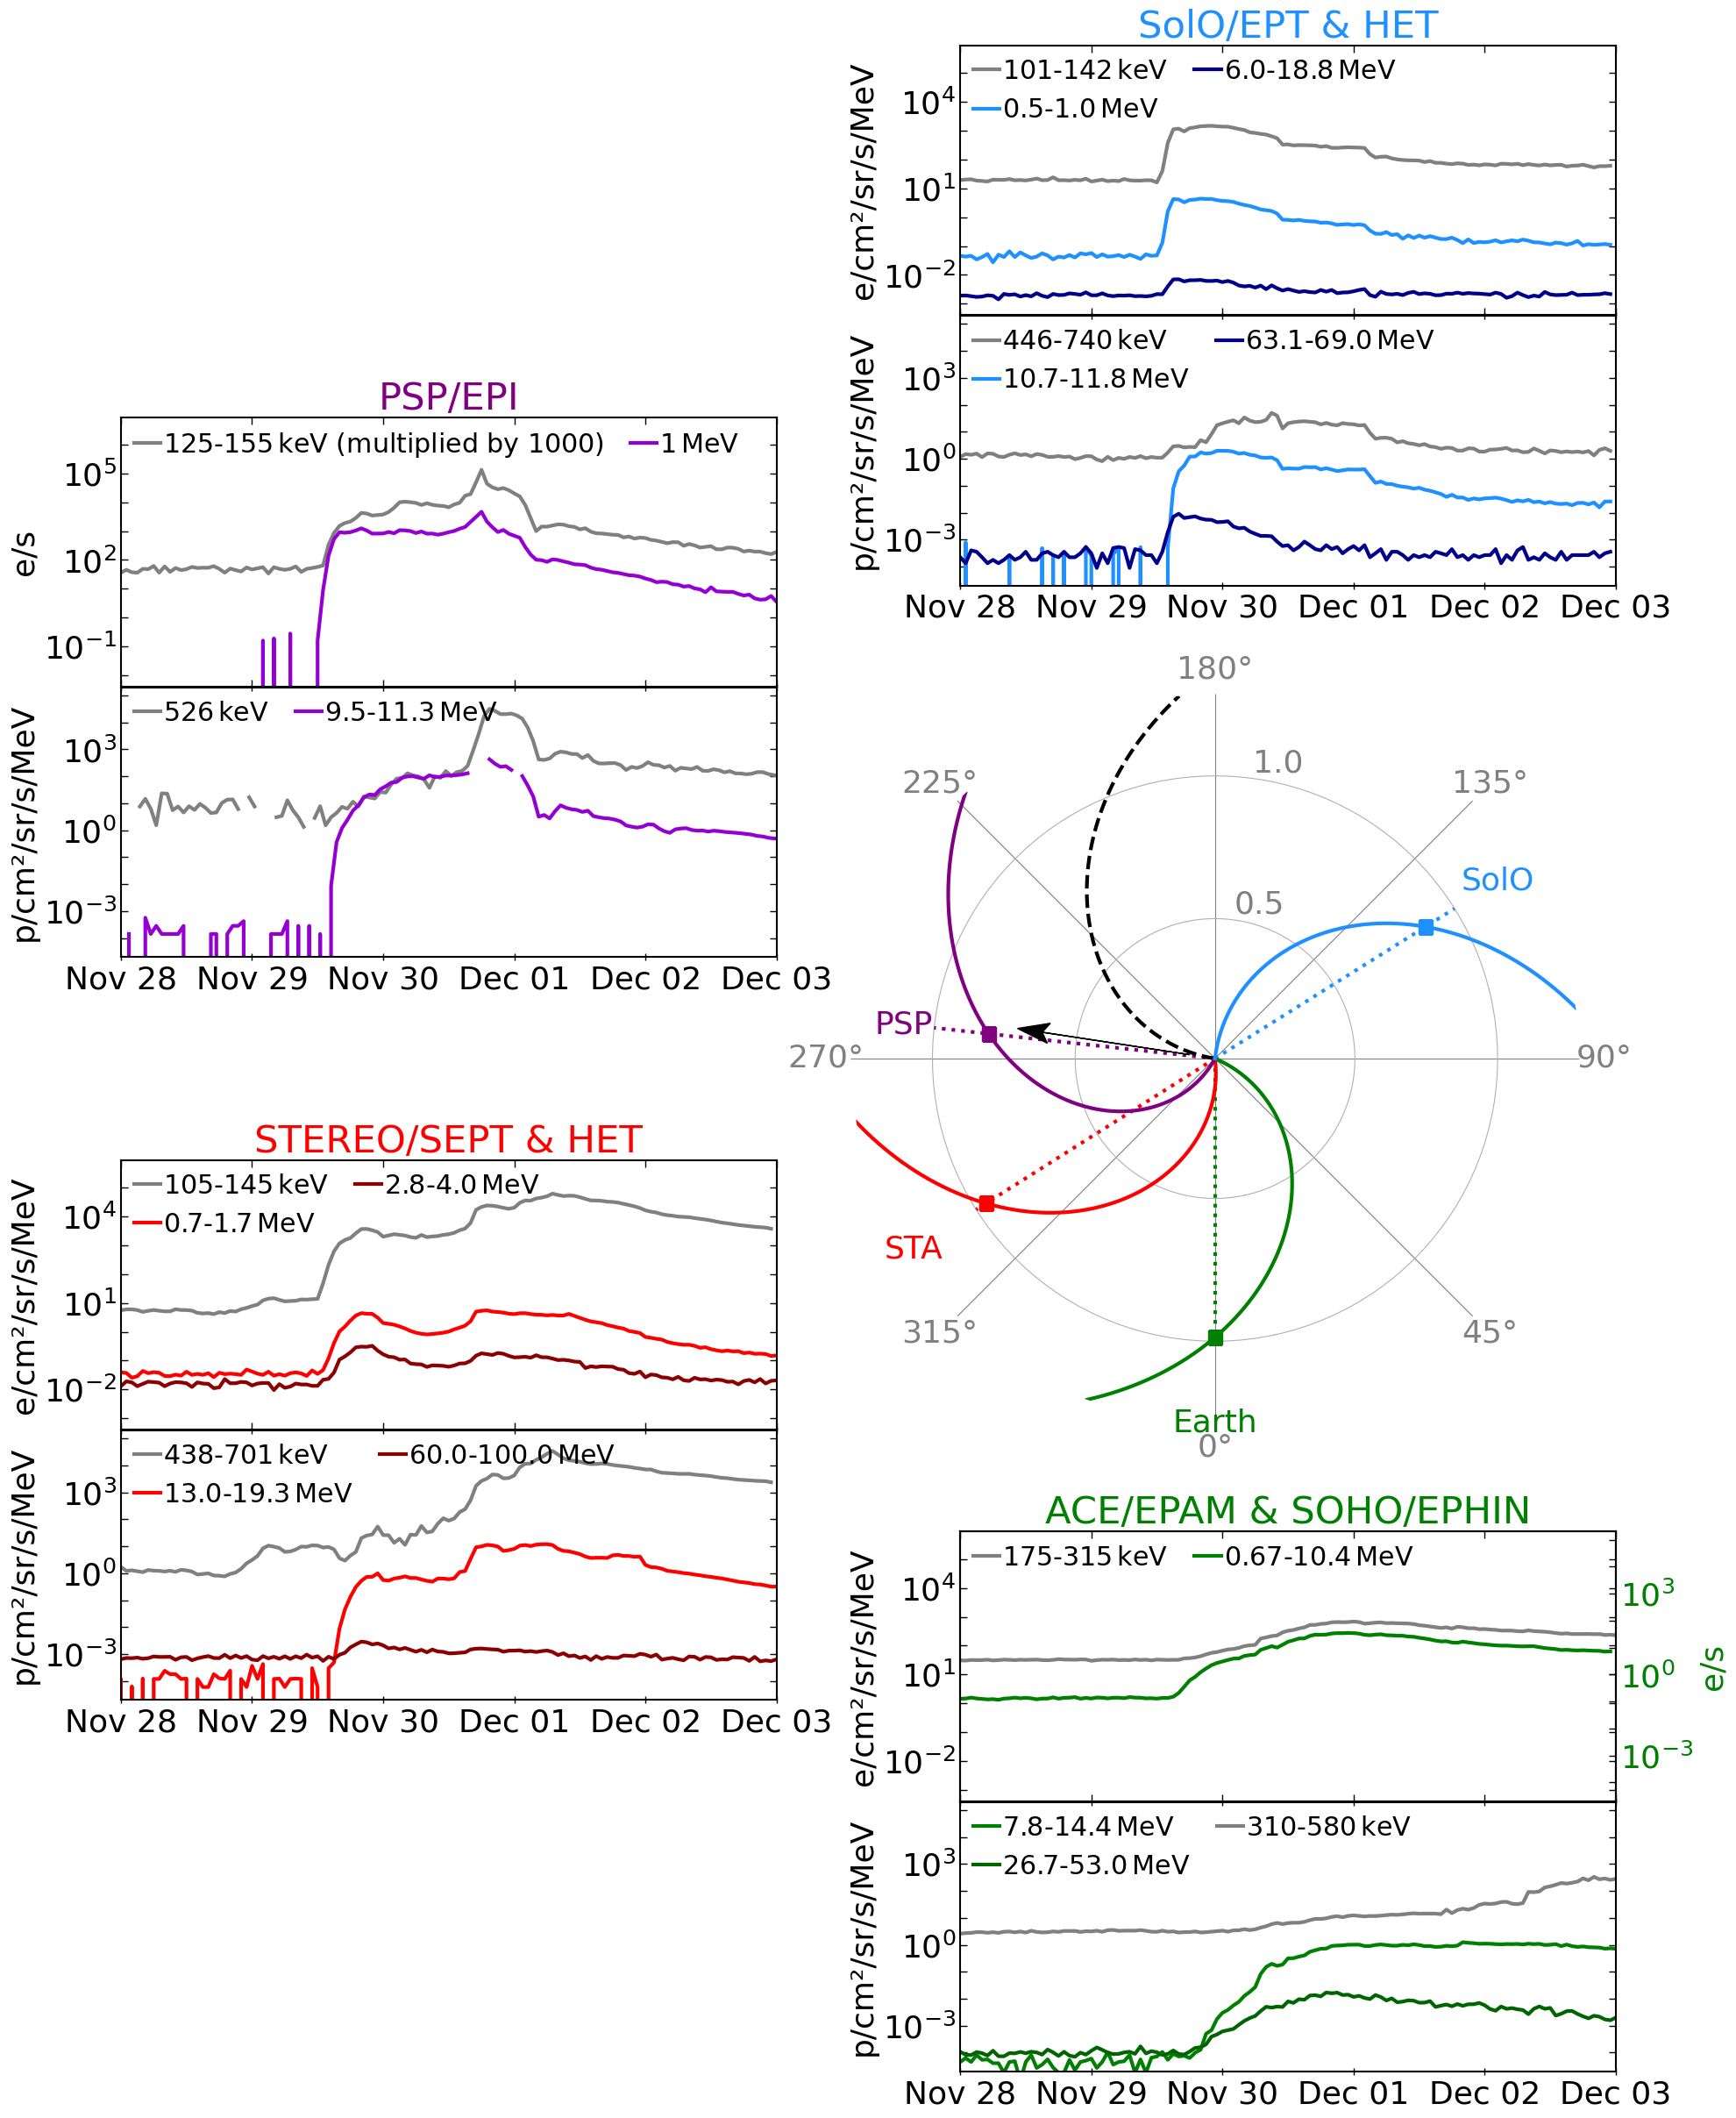
\includegraphics[width = 0.7\textwidth, height = 0.5\textheight]{images/2020-11-29_overview_plot.png}
	\caption{The first wide-spread \acl{SEP} event on Nov 29, 2020. The figure is adapted from \citet{Kollhoff-2021}}
	\label{Fig:SEP_widespread}
\end{figure}

The thorough explanations and summary of the remote-sensing observation of \ac{SEP} in radio, EUV, X-ray channels, the particles injection and transport, composition, charge state, anisotropy and spectra evolution can be found in review papers \citep{reames2013two, Desai_Diacalone2016LRSP, Reames2021LNP}
Instead, in this part we briefly introduce the wide-spread \ac{SEP} and the multiple observation of \ac{SEP}.

Figure \ref{Fig:SEP_widespread} is the first widespread \ac{SEP} of the \ac{SC} 25 happened on 2020 November 29 and observed by \ac{SolO} and simultanously by \ac{PSP}, \ac{STEREO}, \acl{ACE}/\ac{SOHO} near the Earth \citep{Kolhoff2021AA, Kouloumvakos2022AA, Palmerio2022SpWea}. Both relativisitc electons and higher energy protons with energy $>$50 MeV were observed.  The particles in this event spread over a more than 230$^\circ$ longitude regions at 1 au. This SEP is associated with an M4.4 class flare accompanied by \ac{CME}, \ac{EUV} wave and type II/III radio burst. The black arrow in the central panel indicates the location of the active region and the possible location of the central meridian of the \ac{CME}.  Depending on the magnetic connection between \ac{CME} shock and instrument at different locations, as indicated by the colorful line in central panel, the time profiles of particles have different shape. For instance, \ac{PSP} and \ac{STEREO} connect closely to the central meridian, hence the intensity profile shape are similar with the \ac{SEP} we showed in Fig.~\ref{Fig:two_type_SEP}, i.e., abrupt increase with a later peak when the shock reached the s/c location. While Earth is about 166$^\circ$ away from the active region and connect to the west limb of the source, the intensity of the event slowly increases before they peak.

Recently a comprohensive study of the second widespread \ac{SEP} of \ac{SC} 25 occured on 2021 April 17 has been carried out by \citep{dresing202317}. The particles was detected over a more than 210$^\circ$ longitudianl region at 6 locations including four used in the previous event, and \ac{Bepi} as well as Mars, though the Mars observation only provide a observational contrain. Those locations are distributed in different radial distance. \citep{dresing202317} argue that the distinct SEP injections cover a wide range of longitudes might be responsible for this widespread SEP event.

As indicated from the above two examples, the wide spread \ac{SEP} event is a type of event that particles can spread over a large range of longitude ($>$ 200$^\circ$). The shape of particle temperal profiles at different locations, especially if they are far away from each others, varies a lot, which indicate the completely different transport effect and source of particles. 
Therefore one of the most important question of wide spread \ac{SEP} is how the energetic particle spread the heliosphere of such large longitudinal region. Many ideas have been proposed to explain the longitudinal property \citep{Richardson2014SoPh, Dresing2012SoPh,Desai_Diacalone2016LRSP, Reames2021LNP}. The possible mechanism of the large spread SEPs including:
\begin{itemize}
	\item Magnetic connection to an expanding coronal and IP shock \citep{Cliver1995ICRC, Torsti1999JGR, Reames1999, cane2003two, Richardson2014SoPh, Kouloumvakos2019ApJ}: The generally accepted reason of the wide-spread proton and ions which are accelerated in the shocks and released from different shock fronts when connecting to the magnetic footpoint of the observer. Hence the SEP distribution depends on the extend of the shock in the inner heliosphere.

	\item Coronal transport \citep{Reinhard1974SoPh, Newkirk1978JGR}: The process that spread energetic particles from the source region i.e. flare or acitve region, to the remote longitudes in the corona via the divergent magnetic field. 
	\item Multiple particle injections from different source \citep{dresing202317}: The distinct \ac{SEP} injections covering the wide range of longitudes might be responsible for the widespread SEP event.
	\item Cross-field diffusion \citep{Dresing2012SoPh}: The particle perpendicularly transport in the solar wind, which is a slow process compared with parallel transportation along the magnetic field lines. 
	\item EUV waves \citep{Rouillard2012ApJ, Park2013ApJ}: A larger scale disturbances in EUV images which encounter the magnetic foot point on the solar surface when propagating and expanding outward.
	\item Meandering magnetic field lines \citep{Laitinen2016AA, Laitinen2023ApJL}: Associated with turbulence in the solar wind and caused effecient propagation process across the magnetic field lines.
	\item Particle transport to remote longitudes by large-scale magnetic loops \citep{Klassen2018AA, Schrijver2013ApJ} and along the heliospheric current sheet \citep{Battarbee2018ApJ}.
	\item Mixture of the process above.
\end{itemize}

To further clarify the processes leading to the wide spread event, multi-spacecraft observations are essential for determining the properties of widespread SEP events \citep{Kolhoff2021AA}. Previously, major contributions to understanding these events have been made by the combined measurements of \ac{STEREO} mission with its two spacecrafts, and the remote-sensing and in-situ measurements near \ac{L1}. Nowadays, with the new era of spacecraft, including \acl{PSP} \citep{Fox2016SSRv}, \acl{SolO}  \citep{Mueller-2020-SolO}, and \acl{LND} \citep{Wimmer2020SSRv} we have a better oppurtunity to investigate the spectral varitaion, acceleration, transport process and other aspects of wide spread \ac{SEP} events in more detail.

%In the above two example, we have already use multiple instrument to study the \ac{SEP} events. While the history of multiple observation dates back to 

%Nowadays, more and more space-born telescopes have been developed and launched to study the center of our heliosphere and moniter the variation of the plasma environment.  
%Study both in-situ and remote.
%Now - \ac{SOLO} \ac{PSP} and \ac{Bepi},  Mars, STEREO missson, helios mission, new mission from China, \citet{Wang2020Solarring,}India

%A numerous observation and simulation studies have been carried on in the past few decade since the discovery of SEP back to 1950s. The major questions of SEP focus on the origin, acceleration and transport of those high energy particles.\citep{Desai_Diacalone2016LRSP}, which is also the goal of recently two missions \ac{PSP} and \ac{SolO}. 

%=========================================

\section{Galactic cosmic rays}

\begin{figure}[htb]
	\centering
	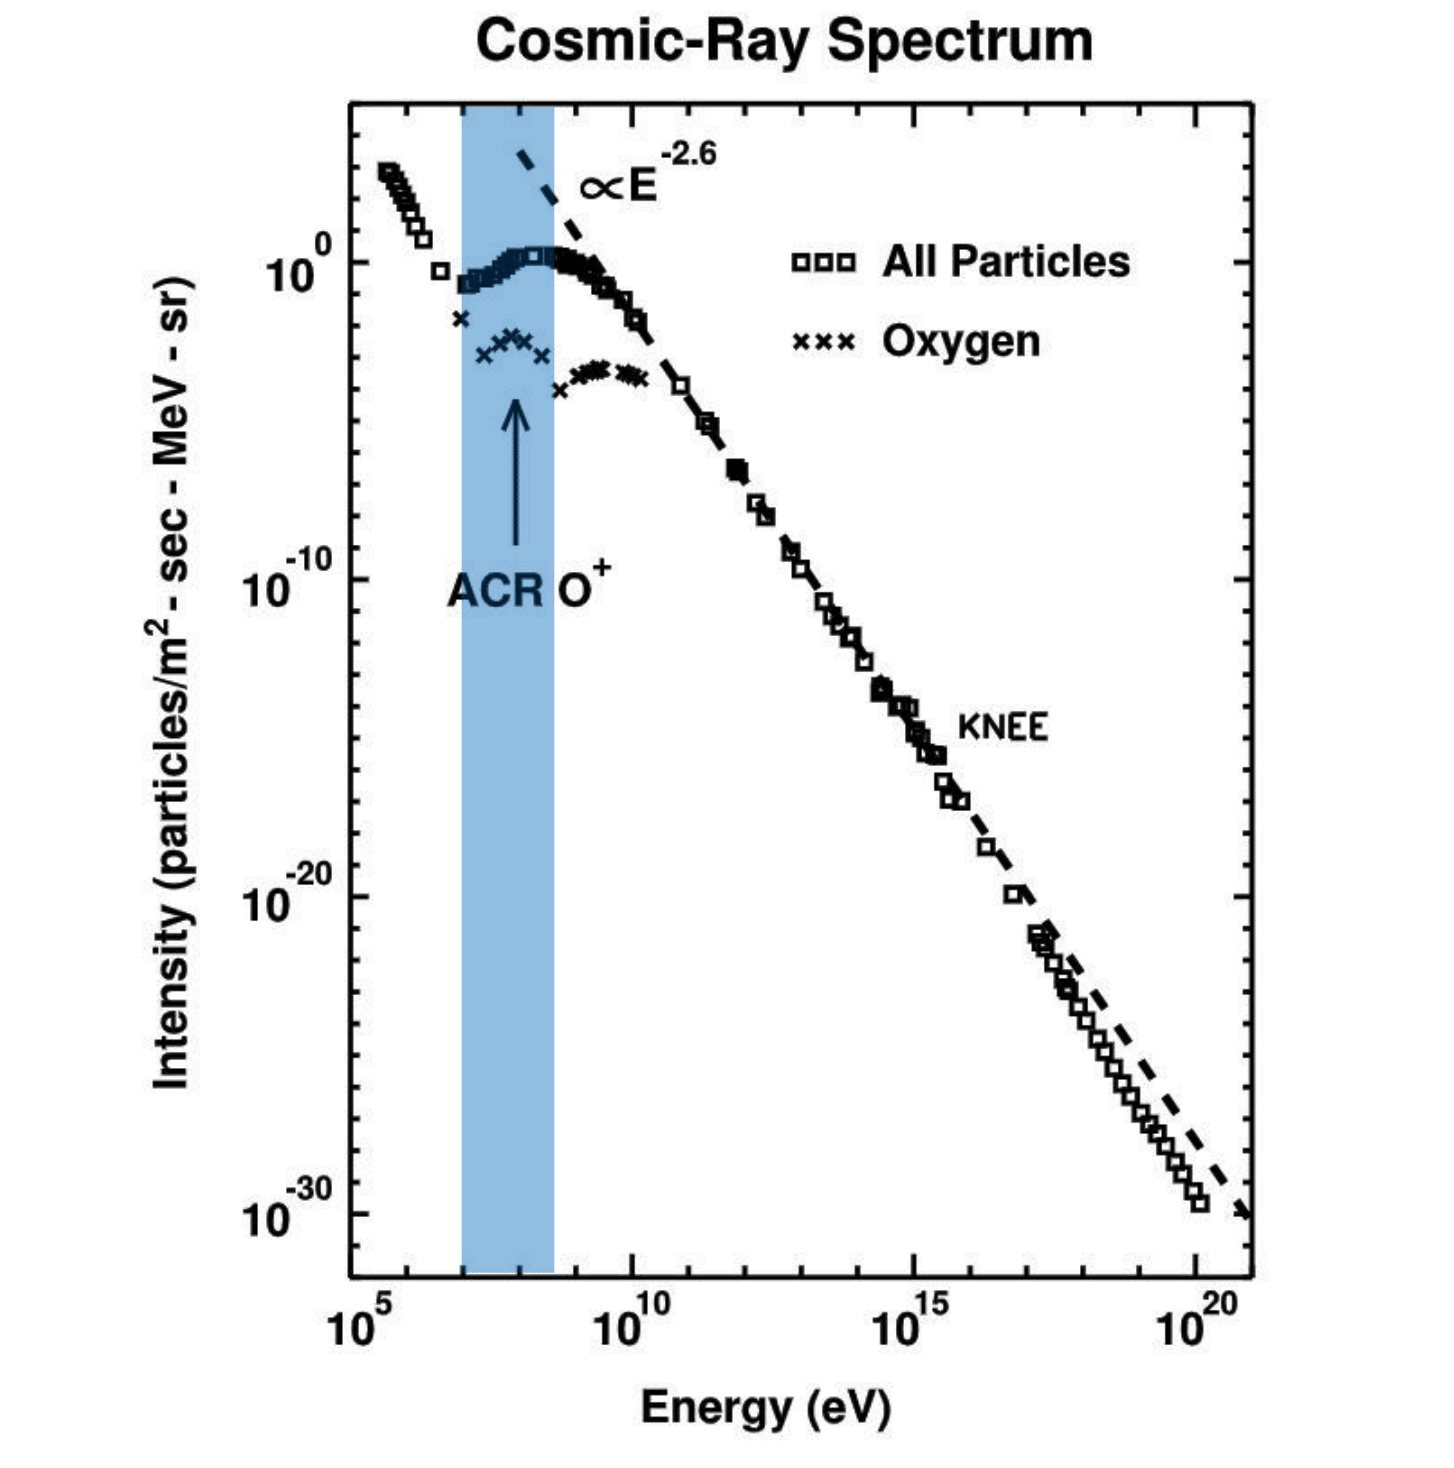
\includegraphics[width = 0.7\textwidth]{images/gcr_spectra_shadow.png}
	\caption[The cosmic ray spectra of all particles at 1 au]{The cosmic ray spectra of all particles and ACR oxygens observed at 1 au. This figure is reproduced from \citet{Giacalone2022SSRv, Giacalone2012SSRv}, which is originally from \citet{Jokipii1990AIPC}.
	The spectrum is plotted in more than 15 orders of magnitude on the energy scale and about 30 orders of magnitude on the intensity scale. Specially it extends the high energy end of Fig.\ref{Fig:Oxygen_spectra_heliosphere}.}
	\label{Fig:Oxygen_spectra_cosmic_ray}
\end{figure}
%\url{https://timeline.web.cern.ch/victor-hess-discovers-cosmic-rays-0}
The first discovery of the \ac{GCR} was made by the Victor Hess in 1912 when he carried on a ballon experiement. The initial purpose of the experiement was to find the source of ionizing radiation in Earth's atmosphere using the electroscope. However, as the ballon climb-up during the experiment, he found that ionization rate measured in the electroscope showed less signicant decrease than anticipated. Such a discrepancy was attributed to the existence of the cosmic rays which increase the radiation in the atmoshphere.

In figure \ref{Fig:Oxygen_spectra_cosmic_ray}, the completed spectrum of the all cosmic particles observed at 1 AU which includes both the \ac{ACR} and \ac{GCR} components is shown. The \acs{GCR} are indicated as empty squares. In the right half of the spectra with energy above 1 GeV, the spectrum could be simply fitted by power a law spectrum with index of about -2.6. The knee of GCR spectra is around few PeV energy and reflects the dominant contribution of hypernovae \citep{Sveshnikova2003AA, Hoerandel2003APh}. The lower energy spectrum  below 1 GeV is shown as a "turn over" which is more complicated and could not be fitted by a signel power law. 

\ac{GCR} consists of multiple energetic particle species spanning a wide range of energy, which are mostly dominated by the proton, about 89\%  and the remains are shared by 10\% helium and a small portal of heavier ions (1\%), electron, positron and antiproton. 
It is believed that \ac{GCR} are mainly originated from the supernova remanent which is a distant location away the sun \citep{Blasi2013AARv2013,Bhattacarjee2000PhR,Fermi1949PhRv} and obtain the energy from the shock waves which is generated from the explosion of supernova \citep{blandford1978particle}.
%When the shock wave travel through the surrounding interstellar gas, the kinetic energy of shock are tranfer to the  (neutral gas?) by the (Fermi-acceleration, ciataion and the acceleration process), Utilimatly, the energetic particle with energy up to 10$^12$ eV are created.

After a long travel, \acp{GCR} arrived the very local bubble which is controled by the sun and its magnetic field.
Before entering the heliosphere, the particles are isotropically distributed in space and nearly constant in time. Because cosmic rays are fully charged, they are deflected by the magnetic field when they propagation in the interstellar space and the directions of those particle are normalized by the strong magnetic field. Hence when they arrived at the space outside of our heliosphere, we obtained an nearly isotropic and constant intensity profile of \ac{GCR}, which is so-called \ac{LISM}.

\ac{LISM} is the modulation boundary and will be modulatined as a function of the position, energy, and time after particle diffusion into the heliosphere. The energy spectrum of \ac{LISM}, especially the lower energy part that could not penetrate heliosphere, have been observed by the voyeger missions after they cross the boundary of solar system and entering the interstellar medium \citep{Stone2013Sci, Cummings2016ApJ,Stone2019NatAs}.
%To model the solar modulation on the particle transportation of GCR spectra, an input particle spectra need to be specifield, which is the so-call LSTM [citaion of LSTM].


When propagating in the heliosphere, cosmic rays are modulated by the solar wind emitting from the sun and its embedding magnetic field periodcally. The relavant process of the solar modulations could be described by a basic \ac{TPE} which is first derived by \citet{Parker1965Pss}. The same equations was also derived by \citet{Gleeson1967ApJ} in a more rigorous way. This equation is based on the motion of charged and particle in the high frequently changed magnetic field and averages over the pitch angle of particle moving in the magnetic field. The precondition of this equation is the reasonable assumption of the isotropically distributed GCRs. The \ac{TPE} gives the phase-space distribution function, $f$ as the function of positions, time and momentum magnetitude. In \citet{Potgieter2013LRSP}, the helispheric \ac{TPE} is rewritten in the following form:

	\begin{equation}
		\underbrace{\frac{\partial f}{\partial t}}_{a} = - ( \underbrace{\boldsymbol{V}}_{b} + \underbrace{\langle v_d \rangle }_{c}) \cdot \nabla f + \underbrace{\nabla \cdot (\boldsymbol{K_s \cdot \nabla f})}_{d} + \underbrace{\frac{1}{3}(\nabla \cdot \boldsymbol{V}) \frac{\partial f}{\partial ln P}}_{e}
		\label{Eq:Transportation_equation}
	\end{equation}

where $f(r, P, t)$ is the cosmic ray distribution as the function of the time t, particle rigidity P and 3-dimension position in the space. Compared with the $\sim$ 11 years solar cycle, the periodcally solar rotation ($\sim$ 27 days) and  the time of the solar wind traveling to the edge of helipshere ($\sim$ 1 years) are short-term variation and can be neglected. Hence the steady-state solution with  $\frac{\partial f}{\partial t} = 0$ (part a of Eq.\ref{Eq:Transportation_equation}) is a reasonable assumption and considered. Terms in the right parts include four effects that are used to describe the variation of the cosmic rays: (b) convection due to the solar wind velocity $\boldsymbol{V}$; (c) drift effects caused by the gradient and curvature of the large-scale \ac{HMF}, which is estimated by a 3D Archimedean spiral \citep{Parker-1958}, $\langle v_d \rangle$ represents the averaged drift velocity; (d) diffusion effects caused by the turbulent mangetic field, with the $\boldsymbol{K}_s$ the symmetrical diffusion tenser; (e) adiabatic energy change and deceleration due to the expansion of the solar wind. 

Since \ac{TPE} is a high non-linear partial differential equation, only a simplified solution of the \ac{GCR} spectra is derived which is called the \ac{FFS}. The \ac{FFS} was first derived by \citet{Gleeson1967ApJ, Gleeson1968ApJ}, which simply depend on the kinetic energy $T$ of particles and the solar modulation potential. Later, a reasonable GCR spectra of the particle with energy above 150 MeV were given by \citet{Gleeson1973ApSS}.
With the development of computer technque and numerical studies, simulation are becoming more and more important in studying the tranporation and solar modulation of the cosmic rays \citep{Jokipii1979ApJ, LeRoux1995ApJ, Manuel2011AdSpR, Potgieter2013LRSP, Vos2015ApJ, Vos2016SoPh,Boschini2019AdSpR, Boschini2022AdSpR, 
Corti2019ApJ, Shen2019ApJ}. 
Commonly used \ac{GCR} models like Badhwar-O'Neill \citep{Oneill2006AdSpR,ONeill2015, Slaba2020SpWea}, CREME \citep{Tylka1997ITNS,Weller2010ITNS} and HELMOD \citep{Boschini2018AdSpR} with the solar modulation and sunspot numbers as input could reproduce the GCR intemnsity and spectra. The model predictions are consistent with the measurements from \ac{ACE} in 1 AU and Voyager probes in the different regions of helisophere \citep{Boschini2019AdSpR}.

\begin{figure}[htbp]
	\centering
	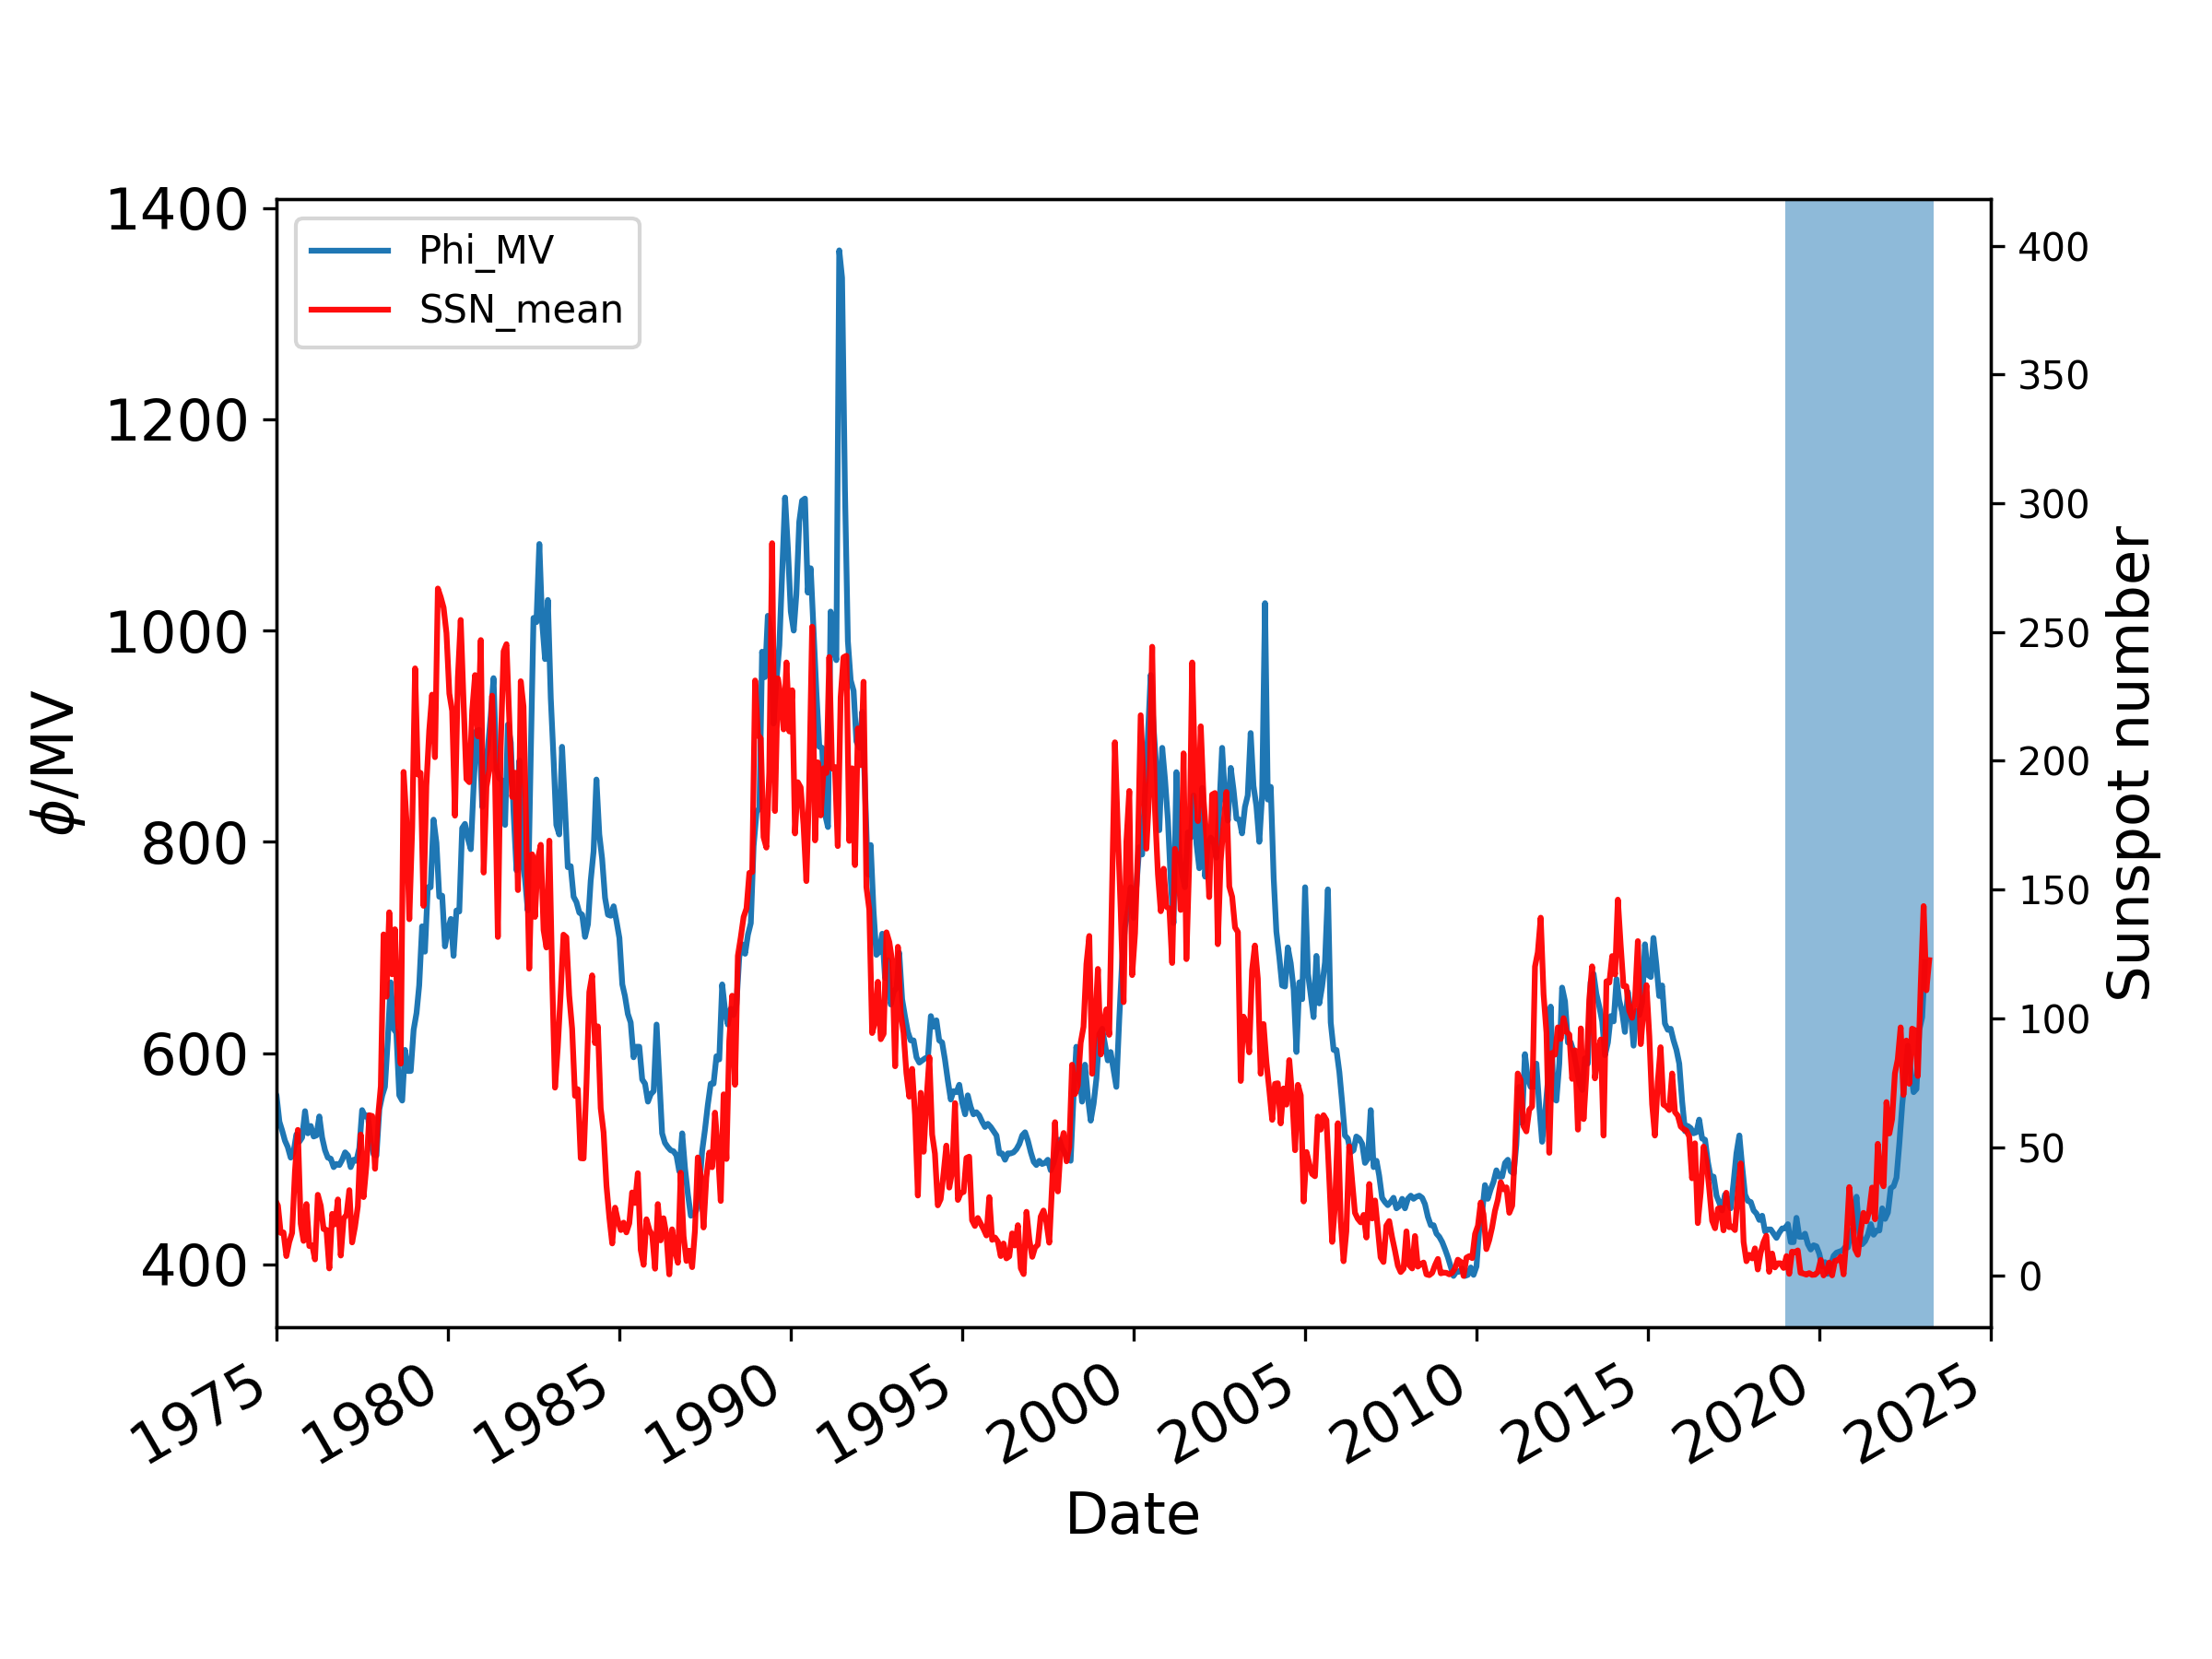
\includegraphics[width = 0.9\textwidth]{images/Solar_modulation.png}
	\caption[Sunspot number and Neutron monitor count data]{Oulu neutron monitor count rate downlowded from \ac{NMDB} measured by Sodankyla Geophysical Observatory of the University of Oulu, Finland and the monthly averaged sunspot number from Solar Influences Data analysis Center (SIDC), Royal Observatory of Belgium, Brussels. The period that we are interested in is marked by the shadow region.}
	\label{Fig:Solar_modulation}
\end{figure}
%\footnotetext{\url{https://www.nmdb.eu/data/}}
%\footnotetext{\url{https://www.sidc.be/silso/datafiles}}

%The solar modulation potential ($\phi$) \cite{Usoskin 2011}, data are downloaded from \url{https://cosmicrays.oulu.fi/phi/phi.html}, 

Figure \ref{Fig:Solar_modulation} shows the monthly averaged sunspot number since 1975 in red and Oulu neutron monitor count rate in blue.
%the solar modulation potential ($\phi$) \cite{Usoskin 2011}.
Sunspot number is a proxy for the solar activities. While the neutron monitor registers the number of high-energy charged particles that strike and penetrate the Earth's atmosphere. The overall variation of the neutron monitor count rate is anti-correlated with the averaged sunspot number.
The count rate peaks when the sunspot number is minimum during solar minimum and vice versa in the solar maximum. The time between two neighbouring solar minimum is about 11 years, which is the period of the solar cycle and caused by the polarity reversal of the solar magnetic field.

Besides the magnetic field reversal, the drift effects play an important role in the 22-year cycle of the intensity of cosmic rays \citep{Jokipii1977ApJ}. Such effects are clearly observed in the temperoal variations.
As shown in Fig.\ref{Fig:Solar_modulation}, during the A $<$ 0 cycle, \ac{GCR} had a more peaked time profile than A $>$ 0 cycle, which have a plateau-like profile. 
This is because in the A $<$ 0 magnetic polarity cycle, the positively (negatively) charged particles drift inwards (outwards) mainly along the equatuorial plane in the heliosphere and drift outward (inwards) through the open mangentic field in the polar region, resulting the sharp change of the intensity. While in the A $>$ 0 cycle, the drift direction of the particle is opposite to the A $<$ 0 cycle, causing the plateau region on the solar minimum. Fig.~\ref{Fig:drift_effect} illustrates the drift effects in the opposite polarity cycles, specifically depicting the drift directions of the positively charged particles such as helium, oxygen.

\begin{figure}
	\centering
	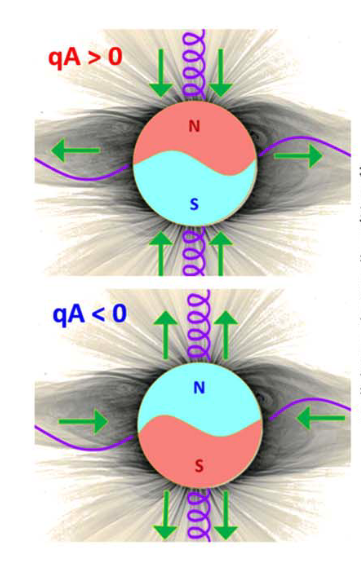
\includegraphics[width = 0.4\textwidth]{images/drift_effect.png}
	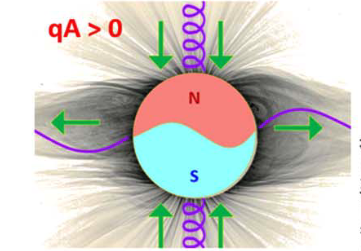
\includegraphics[width = 0.4\textwidth]{images/drift_effect_2.png}
	\caption{The illustration of the drift effects, adapted from the Fig. 4 of \citep{Rankin2022ApJ}}
	\label{Fig:drift_effect}	
\end{figure}

Furthermore, the drift effects which depend on the charge sign and the magnetic polarity are also reflected in the spatial gradient of the cosmic rays, including both \ac{GCR} and \ac{ACR}. In this part, we recap part of the observation of \ac{GCR} particle with energy above hundreds MeV/nuc, though not the focus of this thesis and the details of the \ac{ACR} component will be discussed in the next section.

An evidence of \ac{GCR} latitudinal variation is the obseravtion from Ulysses. \citet{Simpson1995GeoRL, Heber1996GeoRL, Heber1996AA} determined a positive variations with an upper limit of 0.25 \% /$^\circ$  in the A $>$ 0 solar cycle. When the polarity change to negative, the latitudianl gradient was found to change the sign and decrease to a very small value with a maximum of -0.1 \%/$^\circ$ \citep{desimone2011ASTRA, Gieseler2016AA}. It was also found that the solar modulation conditions in the same solar polarity but different solar cycle could affect the latitudinal gradient. \citep{Gieseler2016AA, Vos2016SoPh}. Moreover, the latitudinal gradient of electron was first time determined by \citet{Heber2008ApJ}, which was about 0.2 \% /$^\circ$ and agreed with the proton gradient.

Recently, by revisiting the Helios \citep{} \ac{GCR} proton data, \citet{Marquardt2019AA} found that the radial gradient in the inner heliosphere (0.3 - 1 au) is about 6.6 $\pm$ 4 \% /au, compared with the previous results of 2.5 $\pm$ 0.5 \% /au between 2 and 28 au \citep{Webber1981JGR}. Such a discrepancy indicates that the radial gradients in the inner helioshphere have different bahaviour than that in the outer heliosphere.

%The spatial gradient, including the latitude and radial gradients have already been observed by multiple missions for the region from 1 AU to the edge of the heliosphere in the past few solar cycles, for instance the two Voyager probes, the Ulysses spacecraft, Pioneer and also combined the measurements like PAMELA from L1 point, [citaion]

\section{Anomalous Cosmic Ray}

\ac{ACR} are mostly the singly charged energetic particle dominated the energy range between few meV/nuc to $\sim$ 100 MeV/nuc. \acs{ACR} were firstly discovered by the \acs{IMP} 7 and 8, the missions back to 1970s \citep{Garcia1973ICRC, Hoverstadt1973PhRvL, McDonald1974ApJ}. By analyzing the lower spectra of cosmic rays, the scientist found an "unusual" enhancement of the flux of helium ($<$ 50 MeV/nuc), oxygen and nitrogen ($<$ 20 MeV/nuc) below 100 MeV/nuc. As the oxygen spectrum which is pointed out by the arrow in Figure \ref{Fig:Oxygen_spectra_cosmic_ray} shown, the intensity of lower energy oxygen did not decrease as the energy decrease from hundred MeV/nuc to MeV/nuc, as expected from our understanding of the \ac{GCR} spectrum, but increase instead. Those particles have been known as the \ac{ACR}. \ac{ACR} elements include helium, nitrogen, oxygen, and neon that have been discovered in the inner heliosphere, and Ar and possibly protons that have been found in the outer region of heliosphere \citep{Klecker1995SSRv}.

It is widely believe that ACRs are the high energy interstellar pick-up ions which are accelerated in termination shock of the heliosphere \citep{Fisk1974ApJ}. These pick up ions originate from the intersteallar neutral atoms, which are ionzied by the solar UV and the interaction with solar wind ions when they drift into the heliosphere. Once ionized, the solar wind carries those pick-up ions and transport them to the outer heliosphere, where they are accelerated by the blunt termination shocks \citep{McComas2006GeoRL} and acquire energies of several tens of MeV/nuc. The orientation of termination shock is the most accepted explanation for the \ac{ACR} origin, supported by the current observation of various instrument \citep{McComas2019ApJ, Cummings2019ICRC}.

One of the key chararcteristics of \ac{ACR} is their singly charged nature \citep{Klecker1980GeoRL,Adams1991ApJ, Klecker1995ApJ}. This property suggests a distinct source for \acp{ACR} and seperate it from \ac{GCR} and \acp{SEP}, as well as limits the travel time of \acp{ACR} in the space. Direct measurement of the charge states of ten of MeV/nuc particles is challenging with the current measurement technique. Therefore, in the early stage, most studies relied on the propagtion model to infer the charge states. For example, \citet{Klecker1980GeoRL} reported that the \ac{ACR} oxygens have lower charge states $<$3 by observing the phase leg effects. Later, a clear approach using the Earth's magnetic field as a magnetic spectrometer was employed to determine the charge states. \citet{Adams1991ApJ} and \citet{Klecker1995ApJ} both confirmed the inonic charge states of oxygen, nitrogen and neons at energies in the tens MeV/nuc range, which were found to be equal to 1.

As mentioned and explained earlier, the transport of the cosmic ray in the heliosphere can be described by the \ac{TPE} equation. Various processes are modeled in the equation including diffusion driven by the \ac{HMF} fluctuation, adiabatic energy loss, convection in the expanding solar wind and the drift effects in the large-scale \ac{HMF} which have already been successfully modeled \citep{Parker1965Pss, Jokipii1977ApJ, Jokipii1981ApJ}.

At 1 AU, similar to \acp{GCR}, the intensities of \acp{ACR} are heavily modulated as they traverse the solar wind and globar \ac{HMF}. Figure \ref{Fig:ACR_solarmodulation} illustrates the comparison between the \ac{ACR} oxygen intensity and the neutron monitor count rate which serves as a proxy of the \acp{GCR} variation in the deep space. The \acp{ACR} intensities show clearly the peaked and plateau-shaped profiles which depend on the magnetic polarity over the last two and half solar cycles. Specially, during periods of negative magnetic polarity, particle drift into the heliosphere near the equatorial region along the \ac{HCS} but drift outward from the region near south and north pole. The opposite behavior occurs during the positive polarity \acl{SC}.

%Such a trend is consistent with \ac{GCR} and neutron monitor 
%measurement.


\begin{figure}
	\centering
	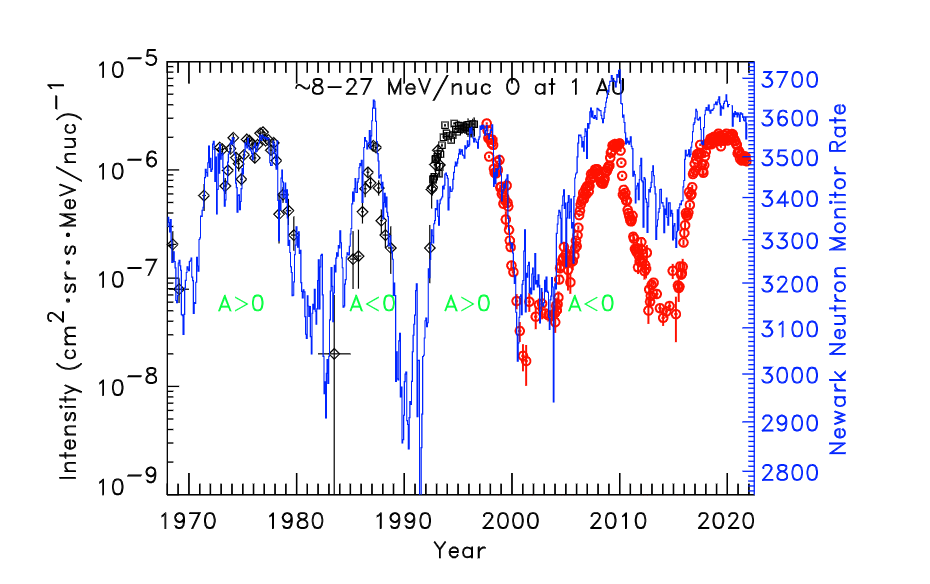
\includegraphics[width = 0.9\textwidth]{images/ACR_solarmodulation.png}
	\caption[Long term variation of \ac{ACR} oxygen and neutron monitor count rate]{ACR oxygen intensity variation with energy between 8 and 27 MeV/nuc at 1 AU measured by ACE/SIS instrument (red) and count rate of Newark Neutron monitor (blue). The blue data points are from the earlier measurements \citep{Mewaldt1993GeoRL}. The plot is adapted from Figure 6 of \citet{Giacalone2022SSRv}}.
	\label{Fig:ACR_solarmodulation}
\end{figure}


As discussed previously, the spatial distribution of the \ac{ACR} along the radial and latitudinal direction contains valuable insight into how the particles transport in the heliosphere and being accelerated out of the helioshphere such as terminaton shock \citep{Rankin2021ApJ}. By quantifying the magnetitude of these gradient, we can estimate and reconstruct the transport process involving drift and diffusion of the \ac{ACR} in the heliosphere. The following general equation is used to model the radial and latitudinal gradients:

\begin{equation}
	\mathrm{ln}(\frac{f_{M}}{f_{E}}) = G_r \Delta R  + G_{\theta} \Delta \theta + C
\end{equation}
where $f_{M}$ is the particle flux measured by spacecraft located away from 1 au and the equatorial plane, like \ac{SolO}, \ac{PSP}. On the other hand, $f_{E}$ is the flux measured at 1 AU by space missions like \ac{SOHO}, \ac{ACE}; $G_r$ and $G_{\theta}$ are the radial and latitudinal gradients, respectively. $C$ is a constant term to account for the additional contributions.

As predicted from cosmic ray transport model, the latitudianl gradient changes sign from positive to negative or vice versa during different polarity \ac{SC}. The observation evidence of latitudinal gradient of in the outer heliosphere were firstly determined by the two Pioneer and Voyager missions \citep{Mckibben1979ApJ, Cummings1987GeoRL, Christon1986JGR}. They found that the latitudinal gradients of 15 Mev/nuc \ac{ACR} helium during solar cycle of A $>$ 0 range from 2.1 to 3.1\% /$^\circ$. In contrast, during A$<$0 \acl{SC} the gradient varied between -2.2 and -1.6 \% /$^\circ$. Moreover, ACR oxygen exhibited an even larger latitudinal gradient ranging from -3.7 to -2.9\%/$^\circ$ \citep{Cummings1987GeoRL}.

The Ulysses mission, operating in the inner heliosphere (below 5 au), significantly expanded our understanding of cosmic ray by providing the polar region measurement of the cosmic rays, thus covering a wider latitude region up to 80$^\circ$. \citet{Lanzerotti1995GeoRL} and \citet{Heber1998JGR} conducted studies during the positive solar mangetic period and found the latitudinal gradient varying between 0.39\%/$^\circ$ and 2.12 \%/$^\circ$. However, during the opposite solar polarity, such gradient reduced by approximately five times to about -0.3 - 0.4 \% /$^\circ$, which is consistent with zero. \citet{Cummings2009GeoRL} concluded that particles could not drift into the inner heliosphere along the \ac{HCS} in this solar cycle. Additionally, a north-south asymmetry of cosmic rays was reported by \citep{Simpson1996ApJ}.

Studies investigating the radial gradients of \ac{ACR} are still ongoing and discrepancies have been found between the recent measurements in the inner heliosphere and the previous studies \citep{Webber1981JGR, Marsden1999AdSpR}. Recent studies by \citet{Rankin2021ApJ, Rankin2022ApJ, Marquardt2018AA}, utilizing different measurements from Helios and \ac{PSP}, have reported a consistent ACR oxygen radial gradient about 45\% /au during A $>$ 0 solar cycle. However this gradient is approximately three times higher than the measurement reported by \citet{Webber1981JGR}. Moreover, \citet{Rankin2022ApJ} reported the radial gradient of ACR helium with energies between 4 - 45 MeV/nuc during the last solar minimum (2018-2020), which was estimated to be approximately 25$\pm$ 5\% /au. Those values are also higher than the prior observations from Pineer, Voyager and Ulysses mission \citep{McDonald2001ICRC, Webber1981JGR, McKibben1989JGR, McDonald1986GeoRL, Cummings1987GeoRL, Cummings1995GeoRL}. The discrepancies observed in the radial gradient of \acp{ACR} still worth to be further investigated, particularly considering the new measurements from \ac{SolO} and \ac{PSP} which are operating below 1 au.


\section{Radiation hazard of energetic particle}


High-energy particles pose a significant threat to human body and electronic hardware in the deep space and on the planetary surface such as Mars and Moon, where effective protection from the atmosphere and inner magnetic field is absent.
These particles have the ability to damage the \ac{DNA} in our cells when they penetrate tissue or organs, even leading to the death cell.
High doses of radiation caused by high-energy charged particle or  neutral parrticle result in Acute Radiation Syndrome (ARS) or Cutaneous Radiation Injuries (CRI), which is a rapid whole-body responce \footnote{\url{https://www.nrc.gov/about-nrc/radiation/health-effects/high-rad-doses.html}}. Furthermore, prolonged exposure to the radiation environment increase the risk of cancer, even after the mission is completerd.

In addition to the health risks for astronauts, the high energy particle can also cause the degradation and damage to instruments and the electronic system onboard the satellite in the space. One of primary reason of the instrument failure is due to the so-called \acp{SEE} which is the change of state of a memory cell or transistor in the electronic devices, induced by the ionizing particles, particularly heavy ions. \acp{SEE} can result in permanent or temporary failure of the electronic systems, potentially leading to the loss of mission. 


% https://www.epa.gov/radiation/radiation-health-effects

The radiation hazard posed by the energetic particles, according to their source, can be seperated into two types: short-term but intense radiation caused by \acp{SEP} and prolonged but lower intensity radiation mainly caused by the \ac{GCR}.
Exposure to intense radiation can lead to acute radiation syndrome, such as nausea and vomiting. While the chronic exposure to the \acp{GCR} radiation environment, although not fatal immediately, can increase the risk of late-term consequence, such as cancer, damage to the central nervous system and many other side effects \citep{Guo2021AARv_rad, cucinotta2006cancer, Kennedy2014LSSR, Iancu2018Frontiers}. 


The variations of radiation dose rate on the Mars surface over the last ten years, are illustrated in Fig.~\ref{Fig:Rad_GCR_radiation}. Several large \acp{SEP} with sufficient energy penetrating the atmosphere of Mars
resulted the increase of dose rate up to few times higher than the pre-event background. Apart from those abrupt enhancements, the overall dose calculated by the \ac{MSL}/\ac{RAD} shows an increasing trend from the solar maximum to the solar minimum during the solar cycle 24. This long term trend is due to the solar modulation on the \ac{GCR} intensity.
Therefore understanding the variations in radiation dose rates is crucial for assess the potential health risks and properly schedule the human activities in the outer space. 


Fig.~\ref{Fig:SEP-radiation_hazard} illustrate the spectra of two famous \ac{SEP} event happened on April 1998 and September 1989. The shadow regions indicate the proton energy that pose the threats on the human activities. The protons of energeis above 150 MeV (red) are considered as hard radiation, which could penetrate 20g/cm$^2$ of aluminium. On the other hand, the soft protons are categorized as particle with energies abve 50 MeV (shown in yellow), which are capable of penetrating spacesuits and the skin of spacecraft \citep{Reames2021LNP}. 

In addition to the radiation we discussed earlier, the secondary particles such as protons, and neutrals generated from the interaction between energetic paritcle and planetary regolith are another signicant contribution to the radiation dose. The secondary protons possess enough energy to penetrate the space suite and cause the radiation hazard \citep{Xu2022FrASS}. While the secondary neutrals are even more detrimental than the charged particles due to its high penetrating ability and high biological effectiveness, despite their lower intensity.
\citet{Spence2013} estimated the amount of radiation hazard caused by the \ac{GCR} and the secondary particles on the lunar surface by conducting the simulation and found secondary particles account for 8.6\% of the overall radiation dose.

In the future, the potential human mission might require longer stay of astronauts on the planetary surface or in the space when traveling to the destination. Hence the probability of the exposure to the radiations, no matter insense or the chronic one is largerly increased. Therefore, properly estimating and understanding the radiation hazard in different situations and locations is crucial and serves as vital preparation for future human mission.



%Apollo mission not affected by the SEP, 


%Earth is protected by atmosphere and magnetosphere
%Mar not, Lunar not.




\begin{figure}
	\centering
	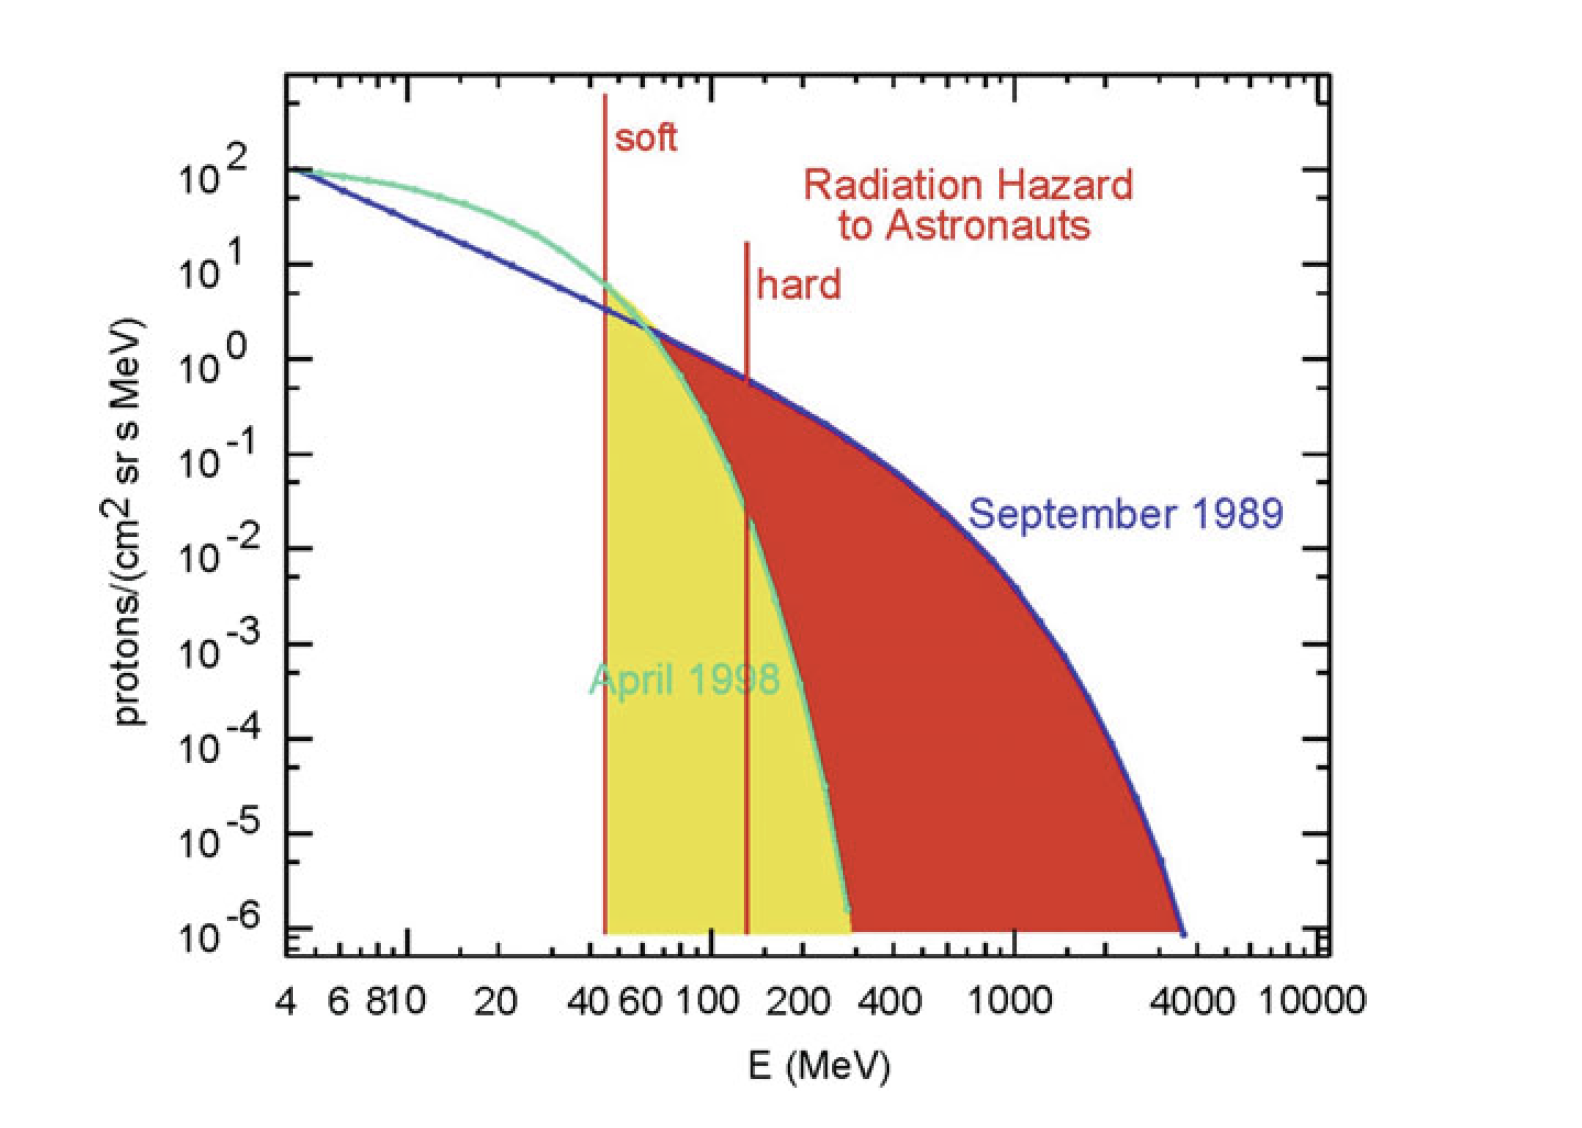
\includegraphics[width = 0.75\textwidth]{images/SEP-radiation_hazard.png}
	\caption[The proton spectra in two SEP events indicating the possible radiation energy]{The proton spectra of two famous SEP events. The shadow regions indicates the energy region of the harmful protons to the instrument and human body. Both "hard" and "soft" spectra threat the human activities. Figure is adapted from \citep{Reames2021LNP}}
	\label{Fig:SEP-radiation_hazard}
\end{figure}


\begin{figure}
	\centering
	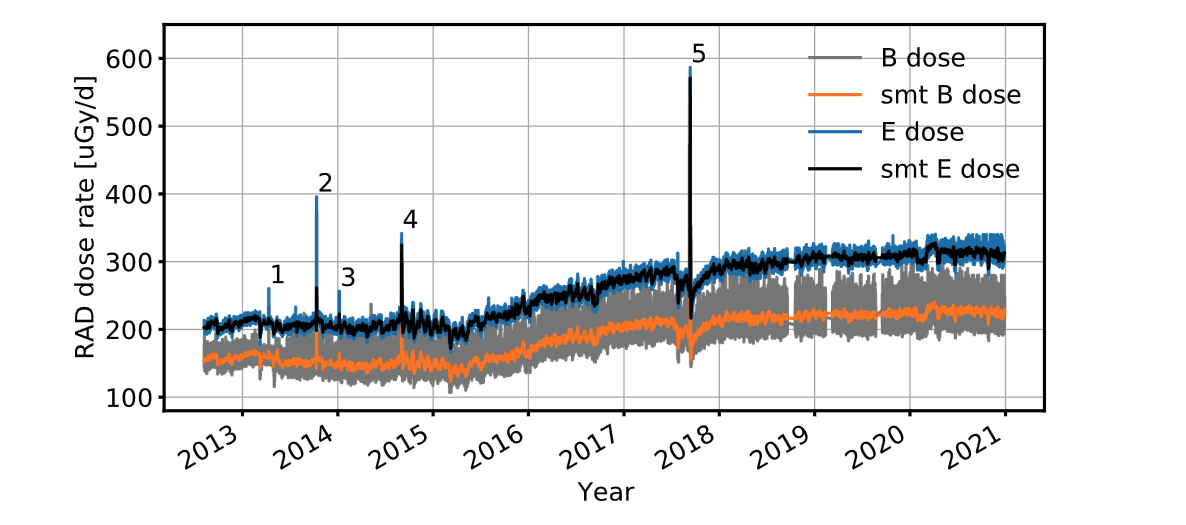
\includegraphics[width = 0.9\textwidth]{images/Rad_GCR_radiation.png}
	\caption[The long term radiation variation measured on the Mars surface]{The radiation dose rates on the Martian surface, measured by the \ac{RAD} in the silicon detector B (grey) and plastic detector E (blue). The daily averaged dose rates of B (smt B dose, orange) and E (smt E dose, grey) overlay the original measurements. Apart from 5 prominent SEPs (number 1-5), the long-term trend of dose rate is correlated with the \ac{GCR} variation. The figure is adapted from \citep{Guo2021AARv_rad}}
	\label{Fig:Rad_GCR_radiation}
\end{figure}



\section{Motivition}

The inspiration of this thesis is from the following three aspects:
\begin{itemize}
	\item New solar cycle: The recently solar minimum have ended in 2020 before the starting of th new \ac{SC} 25. Many observations haved already implied the unusual characteristics of this solar cycle. It is all known that the recent solar minimum have the most quite solar. The \ac{GCR} flux reached historically high levels in the space age \citep{Fu2021ApJS, Xu2022FrASS}, but ACR intensities did not reach such high, record-setting levels \citet{Strauss2023ApJ}. Moreover, the solar activities raised up rapidly and it could be the strongest \ac{SC} since records begin \citet{Nagovitsyn2023SoPh}. The peak of the solar cycle might arrive 1 year earlier than the prediction \citet{McIntosh2020SoPh}. On the other hand, after the solar minimum, the increasing solar eruptions and \ac{SEP} events provide researchers more oppurtunities to study the solar activities and their impact on the Earth and planet.
	\item New mission and new measurements: Over the last few years, several thrilled missions has been successfully launched after extensive preparation, such as \ac{PSP}, \ac{SolO}, \ac{Bepi}, lunar mission like Chang'E series mission, ESA's Jupiter Icy Moons Explorer - Juice, and Chinese missions like CHASE and ASO-S. In this thesis, we focused particularly on the new measurement from \ac{SolO} and \ac{LND}. The former provide the fantastic oppurtunities to study the solar activities in such a close distanc and the latter is the first human mission on the surface of Moon monitoring the radiation environment. The availability of those new observations could enhance our studies of the helioshphere.
	\item Multipoint observations in the heliosphere: With the increasing number of mission deployed in the space, multipoint observations is becoming more and more important and prevalent, enabling comprehensive moitoring of the solar activities at wide spread regions and at different radial distance. 
	
\end{itemize}

Therefore, following the idea of utilizing the new measurements from \ac{SolO} and \ac{LND}, in this thesis, we presents the first  observations of \ac{SEP} from \ac{LND} in Sec.~\ref{chp:LND_SEP}, \ac{GCR} and secondary proton measured on the lunar surface in Sec.~\ref{chp:LND_GCR_albedo}, quite time spectra (\ac{GCR}) measured in the inner heliosphere(Sec.~\ref{chp:SOLO_Quite_time})and the change of the \ac{ACR} helium radial gradient in the new solar cycles (Sec.\ref{chp:ACR_Helium}).
The introduction of the instrument \ac{LND} and \ac{SolO}/\ac{HET} is given in Sec.~.\ref{chp:instruments}. The summary and outlook conclude this thesis. In particular, more detailed information of the \ac{LND} are provided in the Appendix ~\ref{chp:LNDinstrument}

% The exploration of space has witnessed a surge in intensity, with an increasing number of countries aspiring to venture into this domain. Noteworthy examples include NASA's initiation of the Artemis mission, which aims to return to the Moon by 2024. Similarly, China has unveiled its plans to establish a lunar base on the lunar surface by the 2030s, while the European Space Agency (ESA) has also embarked on a lunar lander mission. Most recently, a Japanese lunar lander mission was launched; however, it regrettably encountered failure.

% Under these circumstances, the study of solar energetic particles (SEPs) assumes greater significance. SEPs pose a significant radiation hazard for future human exploration on the lunar surface. The most hazardous SEP events have the potential to induce radiation increases of substantial magnitude.

% SEP events directed towards Earth can become an issue of space weather and
% very energetic events can cause a so-called Ground Level Enhancement (GLE).
% This means that the radiation level on the ground increases which can be seen in
% neutron monitor measurements.